\hfill\break
\justifying
El dar contraste en una imagen implica cambiar el valor de cada uno de los pixeles en una imagen. Este cambio puede ser realizado por la multiplicación o división de los valores de los pixeles en la imagen utilizando una constane.

\hfill\break
\justifying
Utilizando la implementación ofrecida por OpenCV, para el aumento del contraste en una imagen basta asignar un valor positivo a la constante que se evalua en cada pixel. Con la misma lógica, un menor contraste implica un valor de constante positivo menor que 1.

\hfill\break
\justifying
El contraste y el brillo son elementos de las imágenes que pueden ser modificados y que tienen una relación cercana pero no se tratan de lo mismo, aunque suele ser complicado comprender cada uno sin una referencia que comparar.

\hfill\break
\justifying
Cuando en una imagen se ajusta el brillo, el rango entero de valores dentro de la imagen se alza o disminuye respectivamente. Una visualización sencilla de esto es tomando como referencia el histograma de una imagen en niveles de gris. Cuando se aumente al brillo, el histograma mantiene su distribución y forma, pero pareciera se recorre al lado izquierdo por que los valores anteriores de la imagen fueron modificados, aumentados, por la constante.

\hfill\break
\justifying
Cuando se cambia el contraste de una imagen, los tonos medios son eliminados. La imagen tendrá una porcentaje mayor de obscuros o negros, y blancos o resaltados con tonos medios mínimos. Recurriendo a la visualización con el histograma, cuando se contrasta positivamente una imagen, existe un aumento, la distribución de los valores se ensancha hacia los extremos, por lo que visualmente los elementos que se encuentren más separados en el nivel de grises, se verán más claramente cuando comparados. De la misma forma cuando el contraste es negativo, la distribución del histograma tiende a adelgazar y concentrar en un rango menor más valores pixeles.

\begin{lstlisting}[language=Python]
	def contrast(image,alpha:float=1.5,beta:float=0):
		return cv2.convertScaleAbs(image,alpha=alpha,beta=beta)
\end{lstlisting}

\hfill\break
\justifying
La aplicación del contraste con la biblioteca OpenCV se reduce a el manejo de los valores de las constantes $\alpha$ y $\beta$, donde $\alpha$ refiere al contraste y cada vez que se quiera operar directamente en el brillo sin cambiar este, su valor debe ser 1. La $\beta$ opera como la constante encargada de modificar el brillo de la imagen, valores elevados, relativamente, para este parámetro no son tan perjudiciales como puede ser un valor de contraste disparado. Si se desea modificar el contraste unicamente el valor de $\beta$ debe permanecer 0.

\newpage

\begin{landscape}
	\begin{figure}[!h]
		\centering
		\begin{tabular}{cc}
			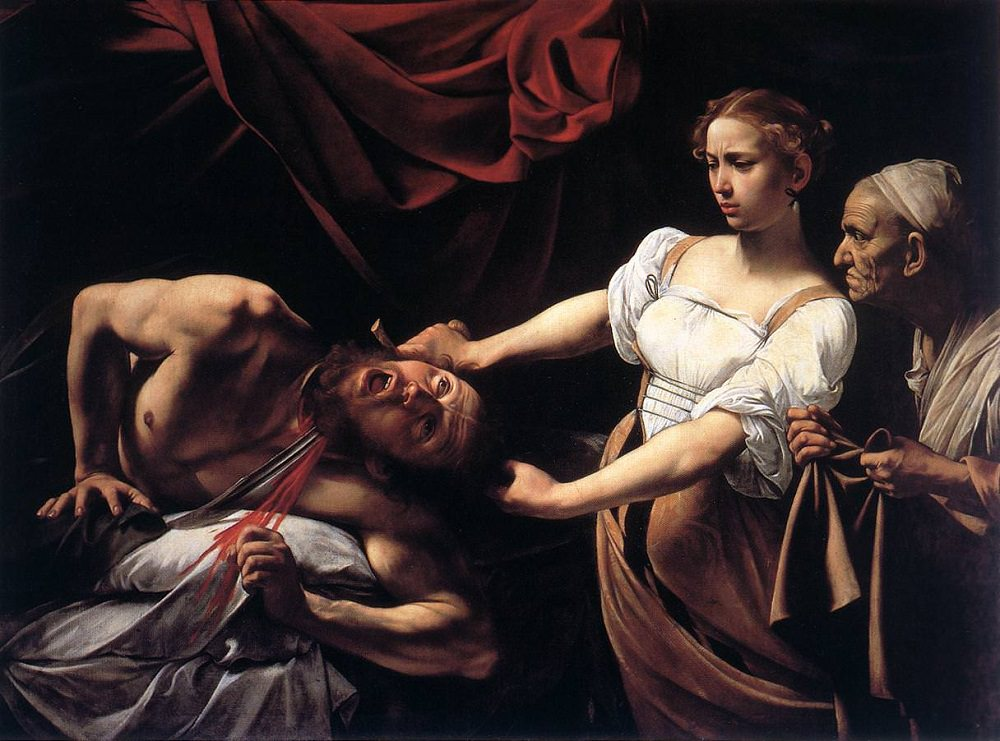
\includegraphics[width=12cm]{Imagenes/caravaggio.jpeg} & 
			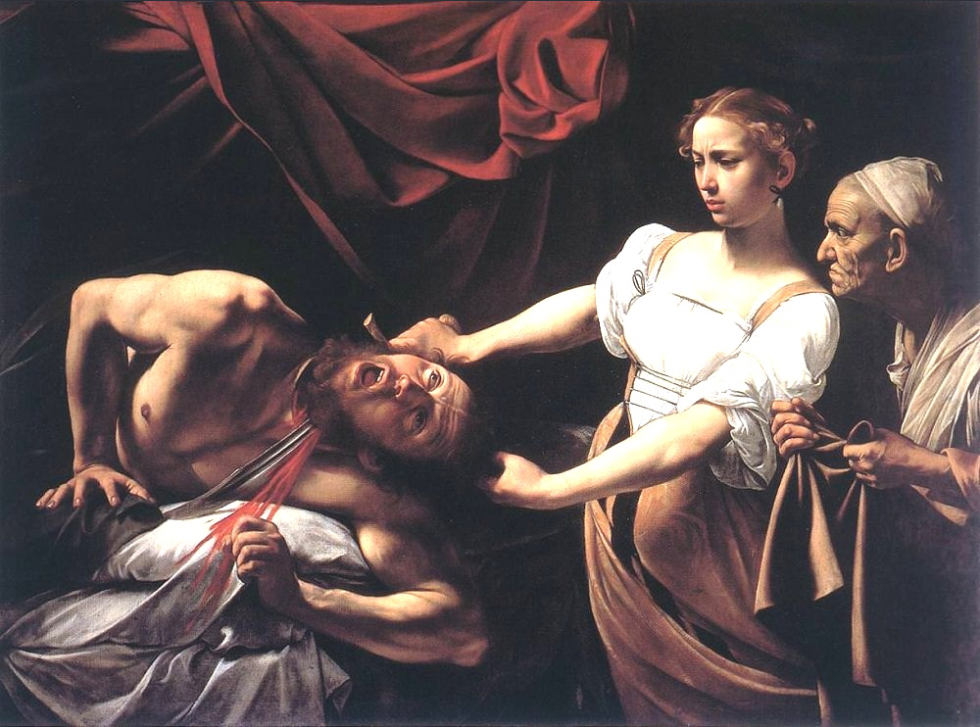
\includegraphics[width=12cm]{Imagenes/Contraste_ambos.png} \\
			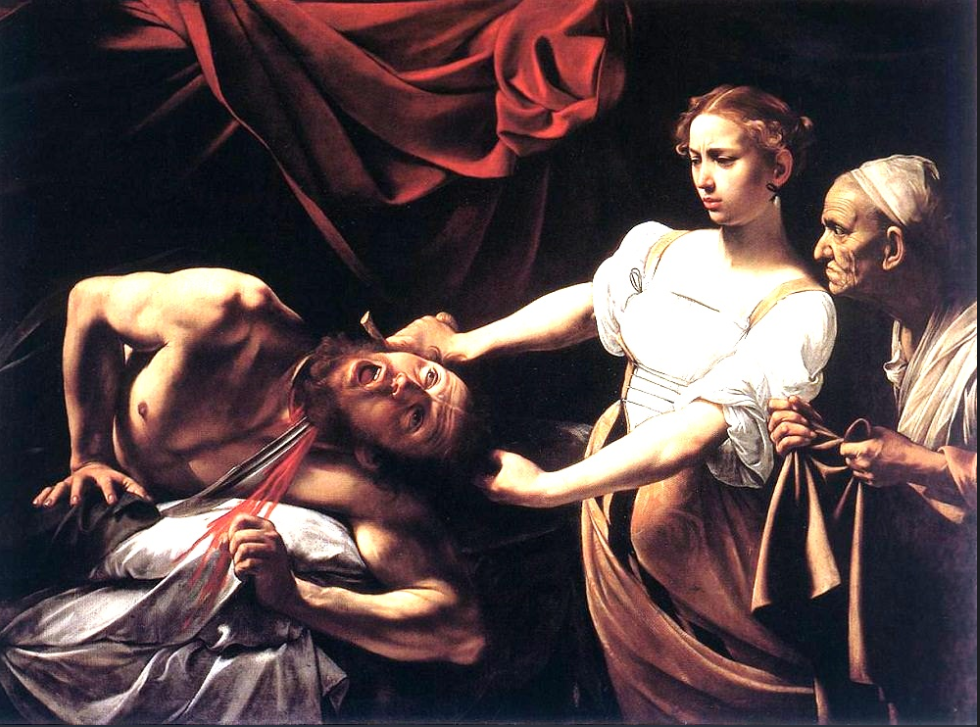
\includegraphics[width=12cm]{Imagenes/Contraste_contraste.png} & 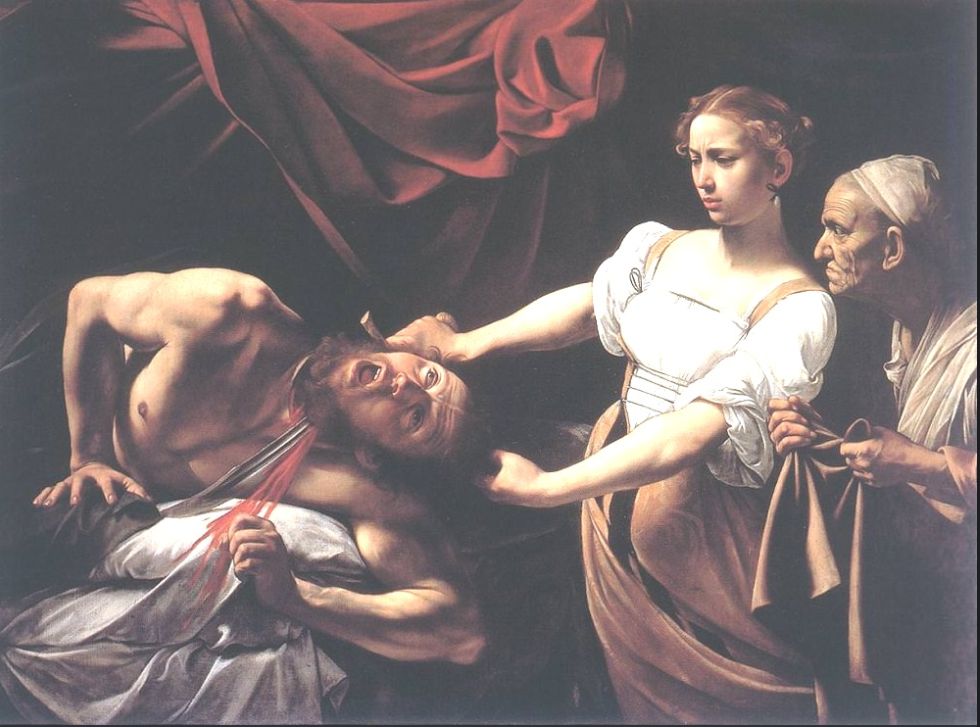
\includegraphics[width=12cm]{Imagenes/Contraste_brillo.png} 
		\end{tabular}
		\caption{1) Imagen original de la pintura 'Judit y Holofernes' de Caravaggio \\ 2) Imagen contrastada y aumentada en brillo respectivamente, con parámetros $\alpha = 1.2$ y $\beta = 30$ \\ 3) Imagen contrastada con $\alpha = 1.7$ \\ 4) Imagen con aumento de brillo $\beta = 70$}
	\end{figure}
\end{landscape}